%%%%%%%%%%%%%%%%%%%%%%%%%%%%%%%%%%%%%%%%%%%%%%%%%%%%%%%%%%%%%%%%%%%%%%%%%%%%%%%%
% TUM-Vorlage: Präsentation - Beispiele
%%%%%%%%%%%%%%%%%%%%%%%%%%%%%%%%%%%%%%%%%%%%%%%%%%%%%%%%%%%%%%%%%%%%%%%%%%%%%%%%

\begin{frame}
	\frametitle{Implementation of Membranes}
	\large
	\begin{itemize}
		\item Membrane is wrapper class around 2d-vector of Particle IDs
		\item Actual Particles still get stored in ParticleContainer
	\end{itemize}
\end{frame}

\begin{frame}
	\frametitle{Implementation of immovable Particles}
	\large
	\begin{itemize}
		\item Set mass of particle to -inf
		\item refactor code to ignore those particles wherever needed (e.g. Thermostat)
	\end{itemize}
\end{frame}

\begin{frame}
	\frametitle{Preparation for Multithreading- Refactoring the Particle Container}
	\large
	Our current implementation of the Cell Data structure (as displayed in Assigment 3):
	\vspace{-0.3cm}
	\begin{itemize}
		\item Particles get stored in one giant vector
		\item Each Cell keeps references to their particles
		\item No sorting or copying takes place
	\end{itemize}
	\vspace{-0.1cm}
	
	\begin{columns}
		\begin{column}{0.5\textwidth}
	\begin{tikzpicture}
		%define constants
		\def\offGrid{3.5}
		\def\offP{2.5}
		\def\arrowStart{0.6}
		\def\arrowEnd{1.9}
		
		\def\scale{1.4}
		
		%draw grid scetch
		\foreach \k in {0,...,3} {
			\draw (\scale*\offGrid+\scale*\k,\scale*0)--(\scale*\offGrid+\scale*\k,\scale*3);
			\draw (\scale*\offGrid +\scale*0,\scale*\k)--(\scale*\offGrid+\scale*3,\scale*\k);
		}
		
		\node[] at (\scale*\offGrid+\scale*0.3, \scale*1.2) {p0};
		\node[] at (\scale*\offGrid+\scale*1.6, \scale*1.2) {p1};
		\node[] at (\scale*\offGrid+\scale*1.3, \scale*1.6) {p2};
		
		%draw datastructure scetch
		
		%particle vector
		\foreach \k in {0,...,2} {
			\node[fill=gray] at (\scale*\offP, \scale*2+\scale*0.5-\scale*\k) {p$\k$};
		}
		%\node at (\scale*\offP, -\scale*0.6) {particles.end()};
		
		\node[] at (\scale*\offP, +\scale*3.5) {particles};
		
		%cells
		\node[] at (\scale*0, +\scale*3.5) {cells};
		
		\node[] at (\scale*0, \scale*2.6 + \scale*0.5) {\vdots};
		\node[] at (\scale*0, \scale*2 + \scale*0.5) {Cell 3};
		\node[] at (\scale*0, \scale*1 + \scale*0.5) {Cell 4};
		\node[] at (\scale*0, \scale*0 + \scale*0.5) {Cell 5};
		\node[] at (\scale*0, \scale*-0.4 + \scale*0.5) {\vdots};
		
		%arrows
		\draw[-triangle 60] (\scale*\arrowStart, \scale*2 + \scale*0.5) -- (\scale*\arrowEnd, \scale*2 + \scale*0.5);
		
		\draw[-triangle 60] (\scale*\arrowStart, \scale*1 + \scale*0.5) -- (\scale*\arrowEnd, \scale*1 + \scale*0.5);
		
		\draw[-triangle 60](\scale*\arrowStart, \scale*1 + \scale*0.5) -- (\scale*\arrowEnd, + \scale*0.5);
		
		%\draw[-triangle 60] (\scale*\arrowStart, \scale*0 + \scale*0.5) -- (\scale*\arrowEnd, -\scale*0.8 + \scale*0.5);
		
	\end{tikzpicture}
\end{column}

\begin{column}{0.5\textwidth}
	\vspace{-4cm}
	
	\begin{itemize}
		\item Sort particle according to cell index of their respective cell
		\item Add size of one cacheline between each cell as padding
	\end{itemize}

	\vspace{-4cm}
	Our changes to avoid false sharing:
\end{column}
\end{columns}
\end{frame}

\begin{frame}
	\frametitle{The Multithreading Oddyssey}
	\PraesentationBildUhrenturm
	%\PraesentationStartseiteFlaggen
\end{frame}

\begin{frame}
	\frametitle{Defining Terminology}
	\large
	Terms necessary to talk about our multithreading approaches efficiently.
	\begin{itemize}
		\item \textbf{Task}: A Task is a pair of cells that should interact with each other. Tasks get represented by pairs of cell indices.
		\item \textbf{Task Model}: The task model defines the data structure that these tasks are stored in.
		\item \textbf{Distribution Strategy}: Many task models require splitting up bundles of tasks into buckets. The distribution strategy defines the strategy used for this splitting process.
	\end{itemize}
\end{frame}


\begin{frame}
	\frametitle{Distribution Strategy}
	\large
	\begin{itemize}
		\item Splitting tasks into even-ish packages is necessary functionality
		\item This problem is np-complete
	\end{itemize}
	
	Approaches we looked at:
	\begin{enumerate}
		\item Round Robin: Assume that every Cell-Interaction has the same weight and distribute them via Round Robin
		\item Greedy distribution: give the next job to the package that has the least work so far
		\item Round Robin Threshold: Give Cell Interactions into one package until the number of interactions surpasses a threshold value (e.g. $10^{4}$ interactions); continue in Round Robin fashion
	\end{enumerate}
\end{frame}
	

\begin{frame}[fragile]
	\frametitle{Approach 1- 1D task model}
	\large
	\begin{itemize}
		\item Store all tasks in one giant "`task pool"' (e.g. a vector)
		\item Schedule freely
		\item Requires reduction
		\item Just one fork and join needed
	\end{itemize}

	\vspace{0.5cm}

	\begin{columns}
		\begin{column}{0.5\textwidth}
			\centering
			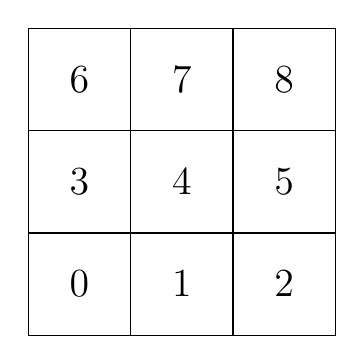
\begin{tikzpicture}[scale=1.3]
			\foreach \x in {0,...,2}{
				\foreach \y in {0,...,2}{
					\draw [draw=black] (\x, \y) rectangle (\x +1 ,\y + 1);
				}
			}
			\node at (0.5,0.5) {\Large 0};
			\node at (1.5,0.5) {\Large 1};
			\node at (2.5,0.5) {\Large 2};
			
			\node at (0.5,1.5) {\Large 3};
			\node at (1.5,1.5) {\Large 4};
			\node at (2.5,1.5) {\Large 5};
			
			\node at (0.5,2.5) {\Large 6};
			\node at (1.5,2.5) {\Large 7};
			\node at (2.5,2.5) {\Large 8};
			\end{tikzpicture}
		\end{column}
	
		\begin{column}{0.5\textwidth}
			\centering
			\vspace{-4cm}
			\begin{lstlisting}
tasks = {(0,1), (1,2,) ...,
	(0,3), (3,6), ...,
	(0,4), (1,5), ...,
	(3,1), (4,2), ...}
			\end{lstlisting}
		\end{column}
	\end{columns}

	
\end{frame}

\begin{frame}[fragile]
	\frametitle{Approach 2- Thread oriented 2D task model}
	\large
	\begin{itemize}
		\item Split up giant "`task pool"' into num\_threads jobs
		\item Use distribution strategy and information unavailable to scheduler (computing cost of each cell interaction) to distribute workload evenly
		\item Give one job to each thread
		\item Requires reduction
		\item Just one fork and join needed
	\end{itemize}



\begin{columns}
	\begin{column}{0.5\textwidth}
		\centering
			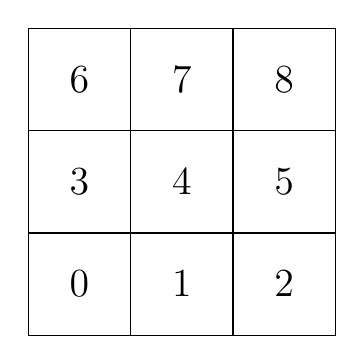
\begin{tikzpicture}[scale=1.3]
	\foreach \x in {0,...,2}{
		\foreach \y in {0,...,2}{
			\draw [draw=black] (\x, \y) rectangle (\x +1 ,\y + 1);
		}
	}
	\node at (0.5,0.5) {\Large 0};
	\node at (1.5,0.5) {\Large 1};
	\node at (2.5,0.5) {\Large 2};
	
	\node at (0.5,1.5) {\Large 3};
	\node at (1.5,1.5) {\Large 4};
	\node at (2.5,1.5) {\Large 5};
	
	\node at (0.5,2.5) {\Large 6};
	\node at (1.5,2.5) {\Large 7};
	\node at (2.5,2.5) {\Large 8};
	\end{tikzpicture}
	\end{column}
	
	\begin{column}{0.5\textwidth}
		\centering
		\vspace{-4cm}
		\begin{lstlisting}
tasks = {{(0,1), (0,3), (3,6) ...},
	{(1,2), (0,4), ...}
	...
}
		\end{lstlisting}
	\end{column}
\end{columns}
	
\end{frame}

\begin{frame}
	\frametitle{Approach 3- Color oriented 2D task model}
	\large
	\begin{itemize}
		\item You need 13 "`lines"' in the Cell-Algorithm to cover all neighbouring cell-interactions
		\item Idea: split up every line into 2 sets of edges to get 26 sets of edges that can be fully parallelized
		\item Fork and join 26 times
		\item No reduction required; no race condition in any of the 26 iterations possible
		\item Forks and joins needed
	\end{itemize}

\begin{columns}
	\begin{column}{0.5\textwidth}
		\centering
		
		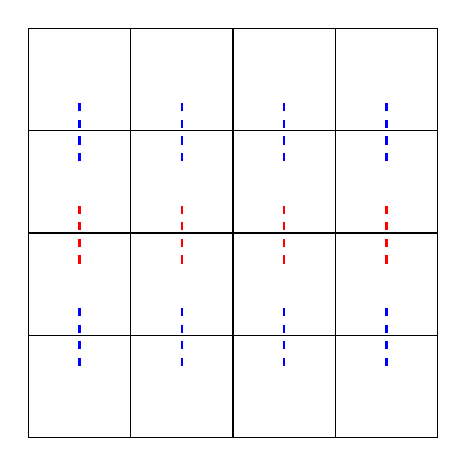
\begin{tikzpicture}[scale=1.3]
			\foreach \i in {0,...,4}{
				\draw (0,\i) --  (4,\i);
				\draw (\i, 0) -- (\i,4);
			}
			
			\foreach \y in {0,2}{
				\foreach \x in {0,...,3}{
					\draw[blue, dashed, thick](\x + 0.5, \y + 0.7) --(\x + 0.5, \y + 1.3);	
				}
			}
			
			\foreach \y in {1}{
				\foreach \x in {0,...,3}{
					\draw[thick, red, dashed, thick](\x + 0.5, \y + 0.7) --(\x + 0.5, \y + 1.3);	
				}
			}
		\end{tikzpicture}
	\end{column}
	
	\begin{column}{0.5\textwidth}
		
		\centering
		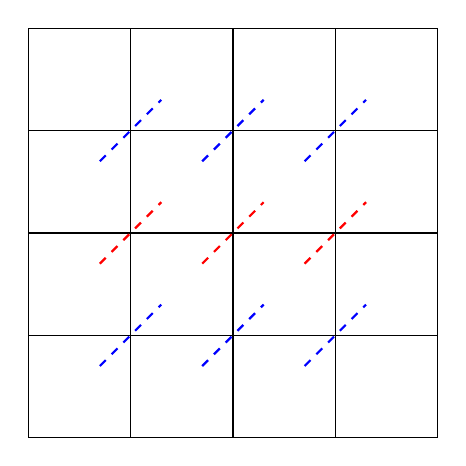
\begin{tikzpicture}[scale=1.3]
			\foreach \i in {0,...,4}{
				\draw (0,\i) --  (4,\i);
				\draw (\i, 0) -- (\i,4);
			}
			
			\foreach \y in {0,2}{
				\foreach \x in {0,...,2}{
					\draw[blue, dashed, thick](\x + 0.7, \y + 0.7) --(\x + 1.3, \y + 1.3);	
				}
			}
			
			\foreach \y in {1}{
				\foreach \x in {0,...,2}{
					\draw[red, dashed, thick](\x + 0.7, \y + 0.7) --(\x + 1.3, \y + 1.3);	
				}
			}
		
			%\foreach \y in {1 ,2, 3, 4}{
			%	\foreach \x in {0,...,3}{
				%		\draw[dashed, thick](\x + 0.7, \y + 0.3) --(\x + 1.3, \y - 0.3);	
				%	}
			%}
		\end{tikzpicture}
	\end{column}
\end{columns}
\end{frame}

\begin{frame}[fragile]
	\frametitle{Approach 3- Color oriented 2D task model}
	
	\begin{columns}
		\begin{column}{0.5\textwidth}
			\centering
			
			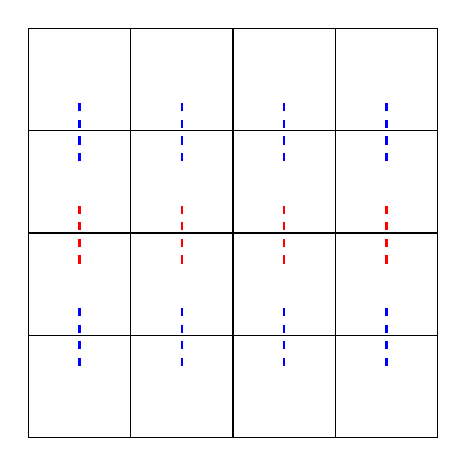
\begin{tikzpicture}[scale=1.3]
				\foreach \i in {0,...,4}{
					\draw (0,\i) --  (4,\i);
					\draw (\i, 0) -- (\i,4);
				}
				
				\foreach \y in {0,2}{
					\foreach \x in {0,...,3}{
						\draw[blue, dashed, thick](\x + 0.5, \y + 0.7) --(\x + 0.5, \y + 1.3);	
					}
				}
				
				\foreach \y in {1}{
					\foreach \x in {0,...,3}{
						\draw[thick, red, dashed, thick](\x + 0.5, \y + 0.7) --(\x + 0.5, \y + 1.3);	
					}
				}
			\end{tikzpicture}
		\end{column}
		
		\begin{column}{0.5\textwidth}
			
			\centering
			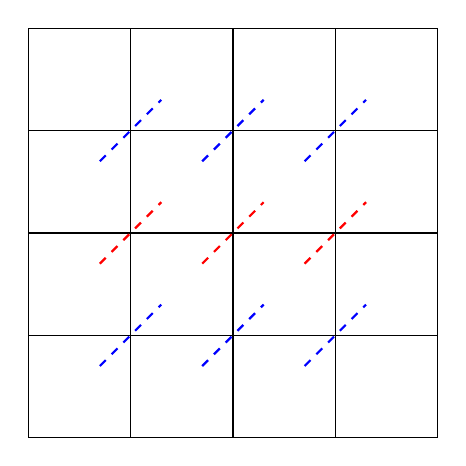
\begin{tikzpicture}[scale=1.3]
				\foreach \i in {0,...,4}{
					\draw (0,\i) --  (4,\i);
					\draw (\i, 0) -- (\i,4);
				}
				
				\foreach \y in {0,2}{
					\foreach \x in {0,...,2}{
						\draw[blue, dashed, thick](\x + 0.7, \y + 0.7) --(\x + 1.3, \y + 1.3);	
					}
				}
				
				\foreach \y in {1}{
					\foreach \x in {0,...,2}{
						\draw[red, dashed, thick](\x + 0.7, \y + 0.7) --(\x + 1.3, \y + 1.3);	
					}
				}
				
				%\foreach \y in {1 ,2, 3, 4}{
					%	\foreach \x in {0,...,3}{
						%		\draw[dashed, thick](\x + 0.7, \y + 0.3) --(\x + 1.3, \y - 0.3);	
						%	}
					%}
			\end{tikzpicture}
		\end{column}
	\end{columns}

	\begin{lstlisting}
				tasks = {{vertical blue tasks},
					{vertial red tasks},
					{diagonal blue tasks},
					{diagonal red tasks},
					{other diagonal blue tasks},
					...
				};
	\end{lstlisting}
\end{frame}
	

\begin{frame}
	\frametitle{Approach 4- 3D task model}
	\large
	\begin{itemize}
		\item Combination of thread oriented and color oriented 2D approaches
		\item Split up tasks into 26 fully parallelizable blocks
		\item Split those blocks into num\_threads jobs; use a distribution strategy to balance workload
		\item No reduction required
		\item Forks and joins needed
	\end{itemize}

\end{frame}

\begin{frame}
	
	\frametitle{Approach Comparison}
	\large
	\setlength\tabcolsep{0.5cm}
	\def\arraystretch{1.5}
	\begin{tabularx}{\linewidth}{>{\hsize=.25\hsize}X|>{\hsize=.25\hsize}X|>{\hsize=.25\hsize}X|>{\hsize=.25\hsize}X}	
		
		1D Tasks & 2D thread tasks
						\begin{tabular}{l|l}
							\hspace{-0.8cm}Greedy & Round Robin\\
						\end{tabular}& 2D colored tasks & 3D tasks  
					\begin{tabular}{l|l}
						\hspace{-0.8cm}Greedy & Round Robin\\
					\end{tabular}\\
		\hline
		\textcolor{black}{Simplest approach} & 
		\textcolor{black}{$+$ Potentially better scheduling than 1D tasks} &
		\textcolor{black}{$+$ Limit for parallelization corresponds to problem given theoretical limit} &
		\textcolor{black}{$+$ Potential to get the best out of both "`2D worlds"'}
		\\ 

		
		
		
		\textcolor{black}{$+$ Just one fork and join needed} & 
		\textcolor{black}{$+$ Just one fork and join needed} &
		\textcolor{black}{$-$ 26 forks and joins needed} &
		\textcolor{black}{$-$ 26 forks and joins needed} \\
		
		\textcolor{black}{$-$ Reduction needed} & 
		\textcolor{black}{$-$ Reduction needed} &
		\textcolor{black}{$+$ No reduction needed}&
		\textcolor{black}{$+$ No reduction needed} \\	
	\end{tabularx}
\end{frame}

\begin{frame}
	\frametitle{Speedup of the 3D task model}
		\begin{figure}
			\centering
			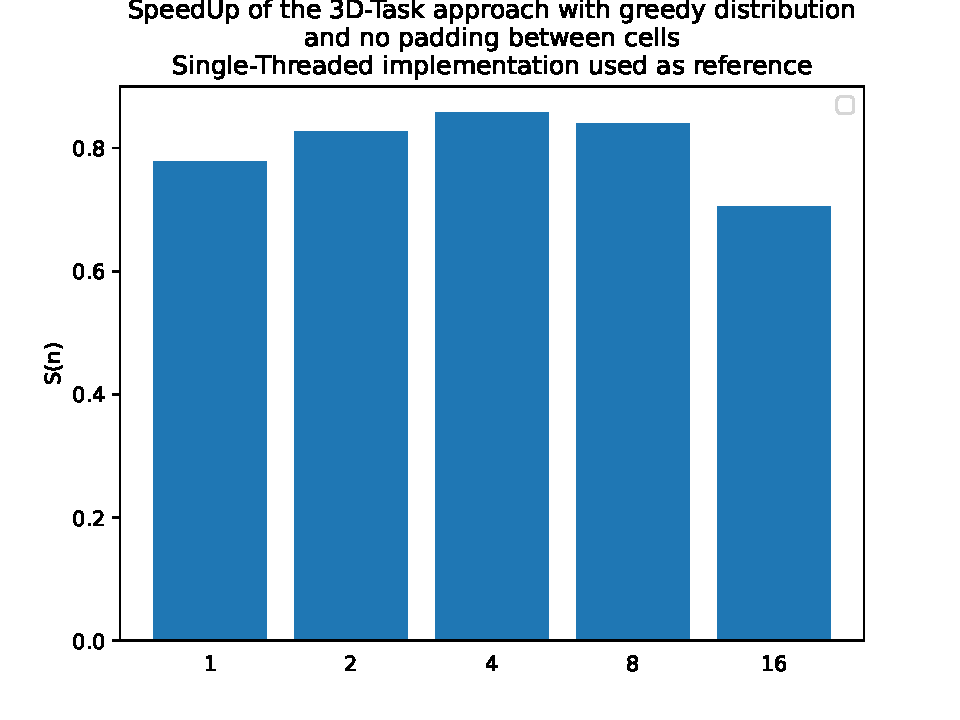
\includegraphics[width=0.6\textwidth]{speedup_3D_st_comp}
			\label{fig:speedup3dstcomp}
		\end{figure}
\end{frame}


\begin{frame}
	\frametitle{What happened?}
	\begin{figure}
		\centering
		\includegraphics[width=\linewidth]{flame_graph_3d_problem}
		\label{fig:flamegraph3dproblem}
	\end{figure}

	\large
\begin{itemize}
	\item As you can see we only use a fraction of our time actually computing forces
	\item The majority of time is spent with OMP overhead
	\item Our conclusion: dividing the workload by $num\_threads\cdot26$ doesn't leave enough tasks in each job	
\end{itemize}
\end{frame}

\begin{frame}
	\frametitle{Speedup of the 1D approach}
	\begin{figure}
		\centering
		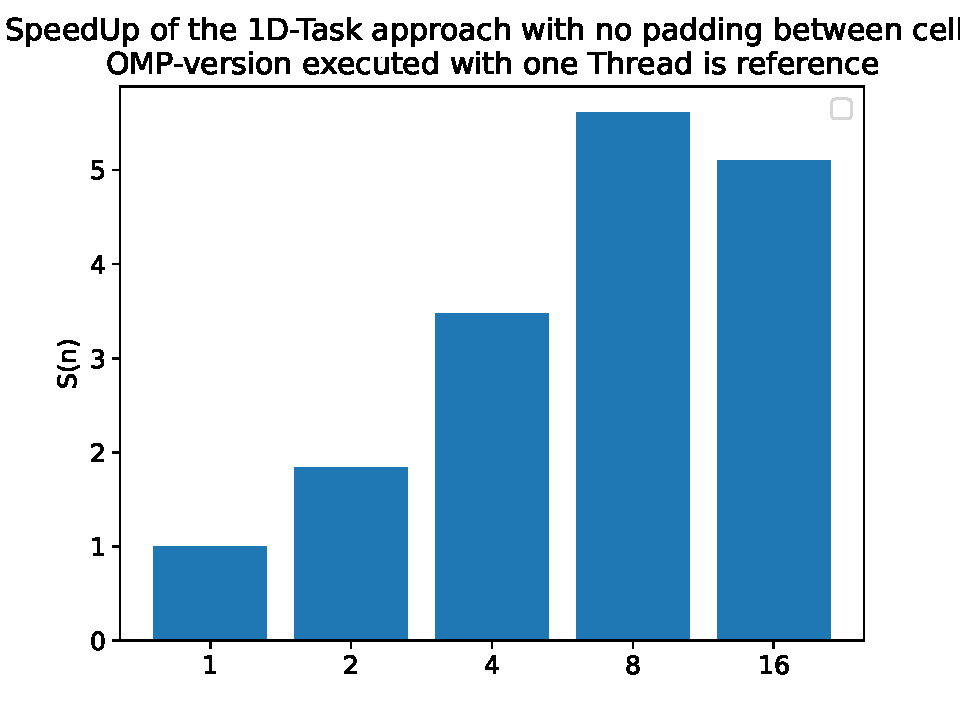
\includegraphics[width=0.6\linewidth]{speedup_1D_omp_comp}
		\label{fig:speedup1dompcomp}
	\end{figure}
	
\end{frame}

\begin{frame}
	\frametitle{Speedups of the 2D approaches}
	\begin{columns}
		
	\begin{column}{0.5\linewidth}
		\begin{figure}
			\centering
			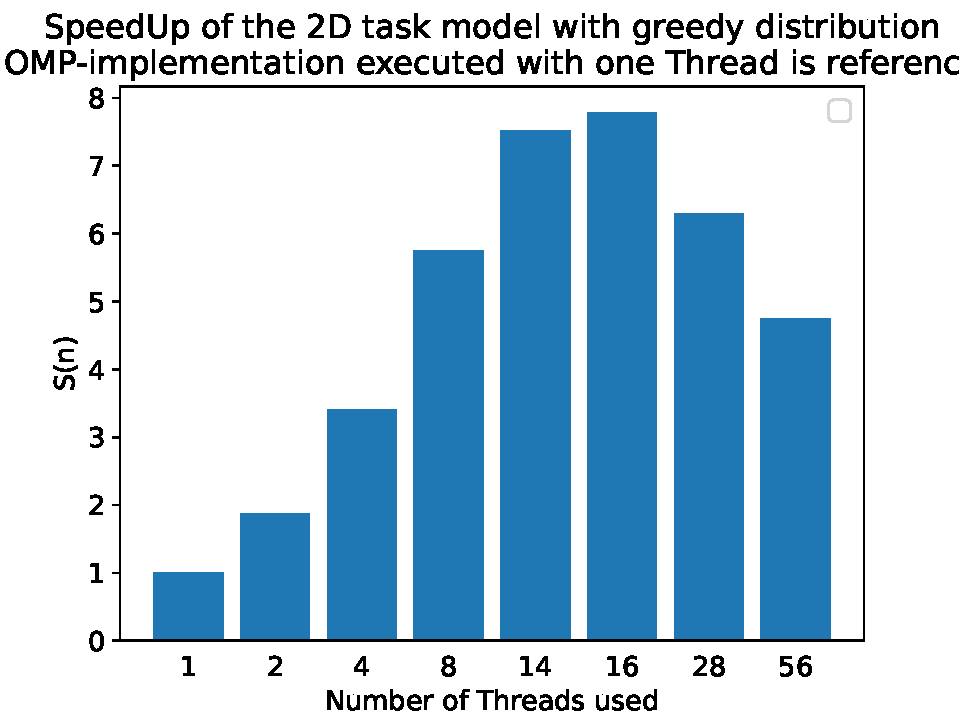
\includegraphics[width=\linewidth]{cluster2DGreedyBarGraph}
			\label{fig:cluster2dgreedybargraph}
		\end{figure}
		
	\end{column}
	
	\begin{column}{0.5\linewidth}
		\begin{figure}
			\centering
			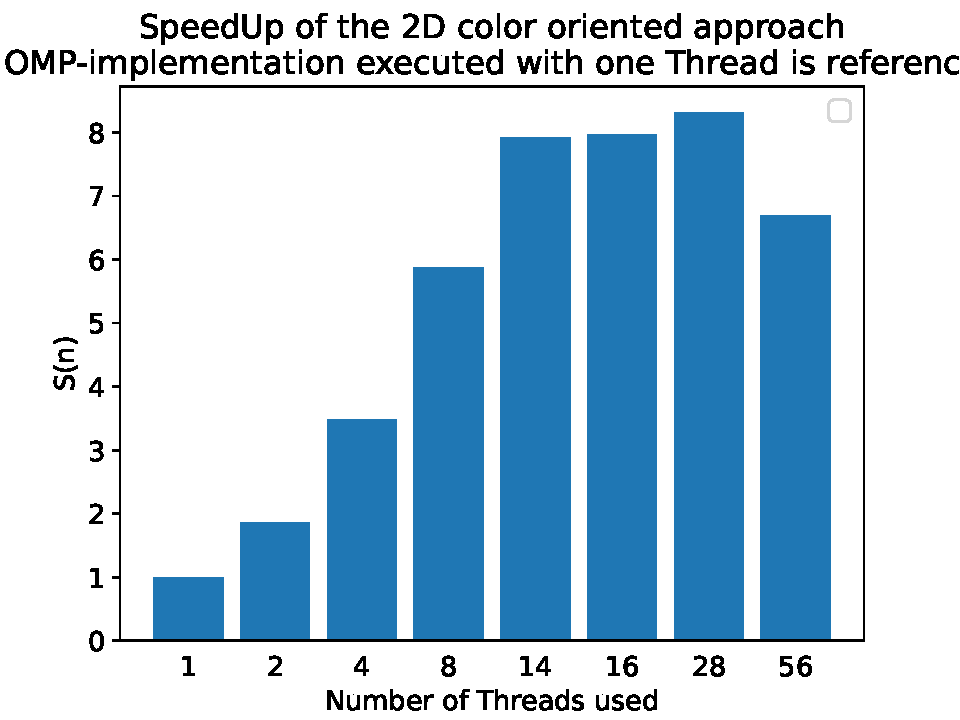
\includegraphics[width=\linewidth]{cluster2DColorBarGraph}
			\label{fig:cluster2dcolorbargraph}
		\end{figure}
	\end{column}
	\end{columns}	
\end{frame}

\begin{frame}
	\frametitle{The price of padding}
	\vspace{0.8cm}
	\begin{columns}
		\begin{column}{0.4\linewidth}
			\large
			\begin{itemize}
				\item As you can see padding adds a measurable overhead
				\item Even in cases where we expected false sharing to occur disabling padding gave a performance boost
			\end{itemize}
			
		\end{column}
		\begin{column}{0.6\linewidth}
			\vspace{-1.6cm}
				\begin{figure}
				\centering
				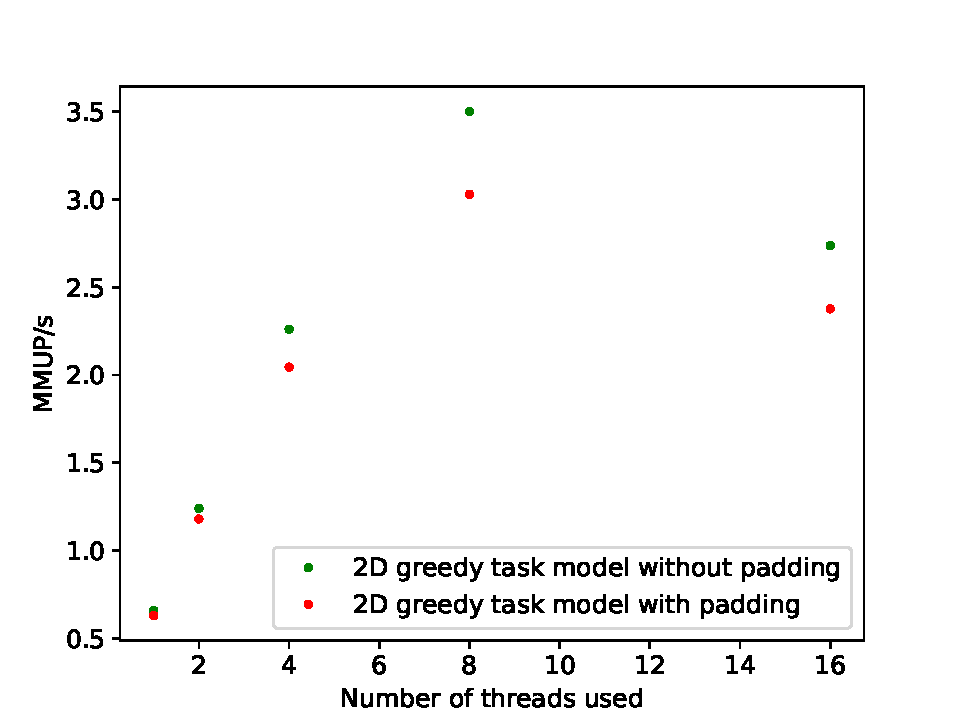
\includegraphics[width=\linewidth]{2DPaddingComp}
				%\caption{}
				\label{fig:2dpaddingcomp}
			\end{figure}
		\end{column}
	\end{columns}
\end{frame}

\begin{frame}
	\frametitle{Comparing distribution strategies}
	
\end{frame}

\begin{frame}
	\frametitle{Why does our Speedup reach a plateau?}
	
\end{frame}

\begin{frame}
	\frametitle{NanoFlow}
	
\end{frame}




\begin{frame}
	\frametitle{Thermostat}
	\begin{figure}
		\centering
		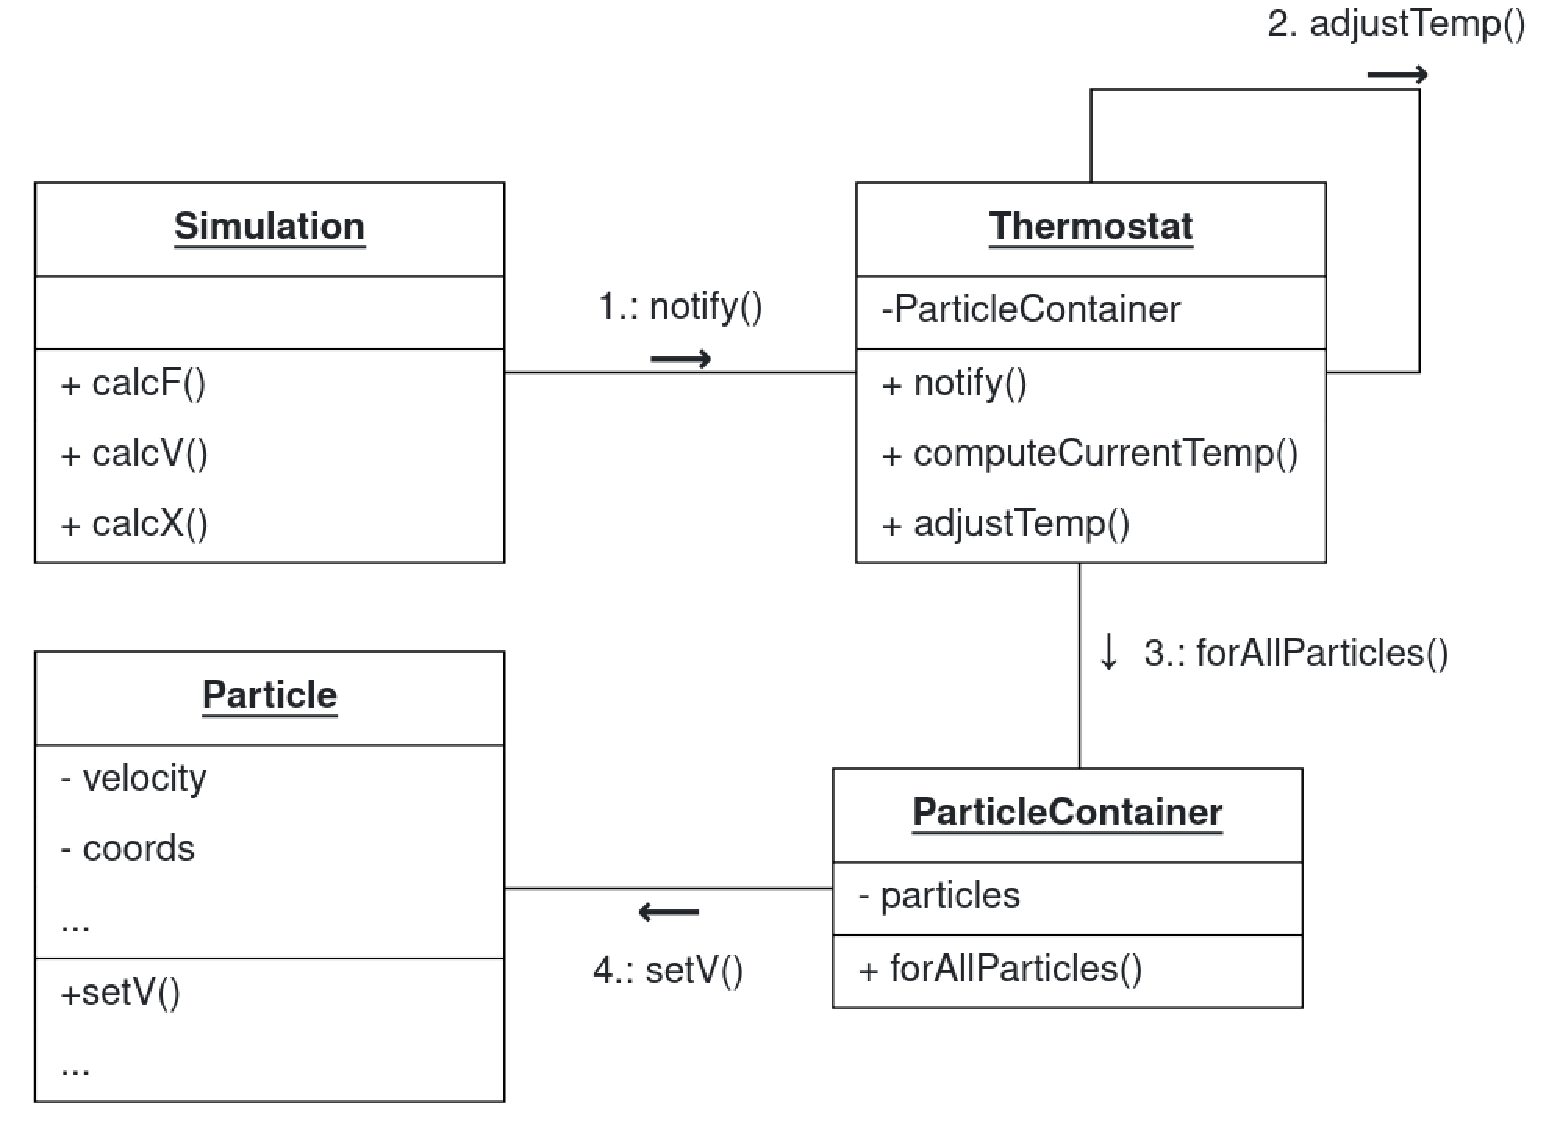
\includegraphics[width=0.55\linewidth]{ThermoComm}
		%\caption{}
		\label{fig:thermocomm}
	\end{figure}
\end{frame}
\begin{frame}
	\frametitle{Adapting ParticleContainer for periodic bounds}
	\large
	Idea:\\
	\begin{itemize}
		\item Provide virtual cells around the actual domain for anyone who needs it
		\item Existence of additional cells is invisible with old interface
	\end{itemize}
	
	\begin{columns}
		\begin{column}{0.6\textwidth}
			\vspace{-5cm}	
			\begin{figure}
				\centering
				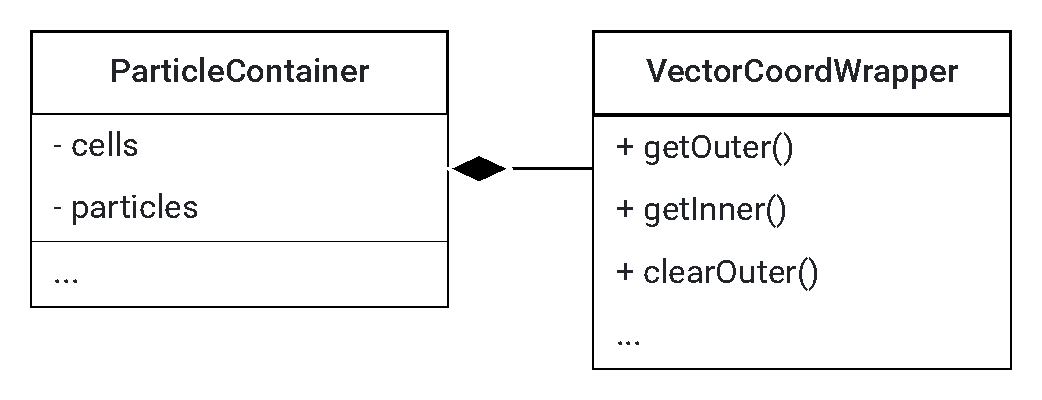
\includegraphics[width=\linewidth]{VectorCoordWrapper}
				\label{fig:vectorcoordwrapper}
			\end{figure}
		\end{column}
		
		\begin{column}{0.3\textwidth}
			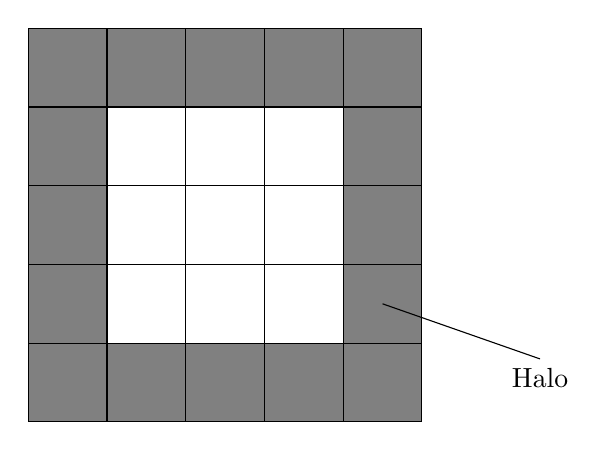
\begin{tikzpicture}
				\foreach \x in {1,...,3}{
					\foreach \y in {1,...,3}{
						\draw [draw=black] (\x, \y) rectangle (\x +1 ,\y + 1);
					}
				}
				\foreach \x in {0,...,4}{
					\filldraw [fill=gray, draw=black] (\x, 0) rectangle (\x +1 ,0 + 1);
					\filldraw [fill=gray, draw=black] (\x, 4) rectangle (\x+1, 4+1);
				}
			
				\foreach \y in {1,...,3}{
					\filldraw [fill=gray, draw=black] (0, \y) rectangle (0+1 , \y + 1);
					\filldraw [fill=gray, draw=black] (4, \y) rectangle (4+1, \y+1);
				}
			
				\draw [below] (4.5,1.5) -- (6.5, 0.8) node[below] {Halo};
			\end{tikzpicture}
		\end{column}
	\end{columns}


	
	
	
\end{frame}

\begin{frame}
\frametitle{Boundary conditions}
\large
Idea:
\vspace{-0.5cm}
\begin{enumerate}
	\item Temporarily move all particles next to Boundary of the other side
	\item Let Neighbouring cells interact
\end{enumerate} 

%\resizebox{0.5\textwidth }{0.5\textheight }{
	\begin{tikzpicture}[scale=1.3]
	%define constants
	\def\xLargeArrow{4.5}
	\def\yLargeArrow{1.5}
	\def\LargeArrowLength{2.5}
	\def\offSGrid{7.5}
	\def\arrowStart{0.6}
	\def\arrowEnd{1.9}
	
	\def\scale{1.4}
		
	%draw left grid
	\foreach \y in {0,...,2} {
		\filldraw [fill=green, draw=black] (0, \y) rectangle (0 + 1 ,\y + 1);
	}
	\foreach \x in {1,...,3}{
		\foreach \y in {0,...,2}{
			\draw [draw=black] (\x, \y) rectangle (\x +1 ,\y + 1);
		}
	}
	
	\fill (0.2,1.4) circle[radius=2pt];
	\fill (2.8,1.4) circle[radius=2pt];

	%arrow in between
	\draw[->, line width = 1mm] (\xLargeArrow, \yLargeArrow) -- (\xLargeArrow + \LargeArrowLength, \yLargeArrow);
	

	%draw right grid with left row put to the right
	\foreach \y in {0,...,2} {
		\filldraw [fill=green, draw=black] (\offSGrid + 3, \y) rectangle (\offSGrid + 3 + 1 ,\y + 1);
	}
	\foreach \x in {0,...,2}{
		\foreach \y in {0,...,2}{
			\draw [draw=black] (\offSGrid + \x, \y) rectangle (\offSGrid + \x +1 ,\y + 1);
		}
	}

	
	\fill (\offSGrid + 3 + 0.2,1.4) circle[radius=2pt];
	\fill (\offSGrid - 1 + 2.8,1.4) circle[radius=2pt];
	
	%arrows
	\draw[-triangle 60] (\offSGrid + 3.5, 1.5) -- (\offSGrid + 2.5, 1.5);
	\draw[-triangle 60] (\offSGrid + 3.5, 1.5) -- (\offSGrid + 2.5, 2.5);
	\draw[-triangle 60] (\offSGrid + 3.5, 1.5) -- (\offSGrid + 2.5, 0.5);
	
	
	\end{tikzpicture}
%}

\end{frame}

\begin{frame}
	\frametitle{The result}
	%TODO: insert video
	\begin{figure}[h!]
		\centering    
		\movie[label=show3,width=0.7\textwidth,poster
		,autostart,showcontrols,loop] 
		{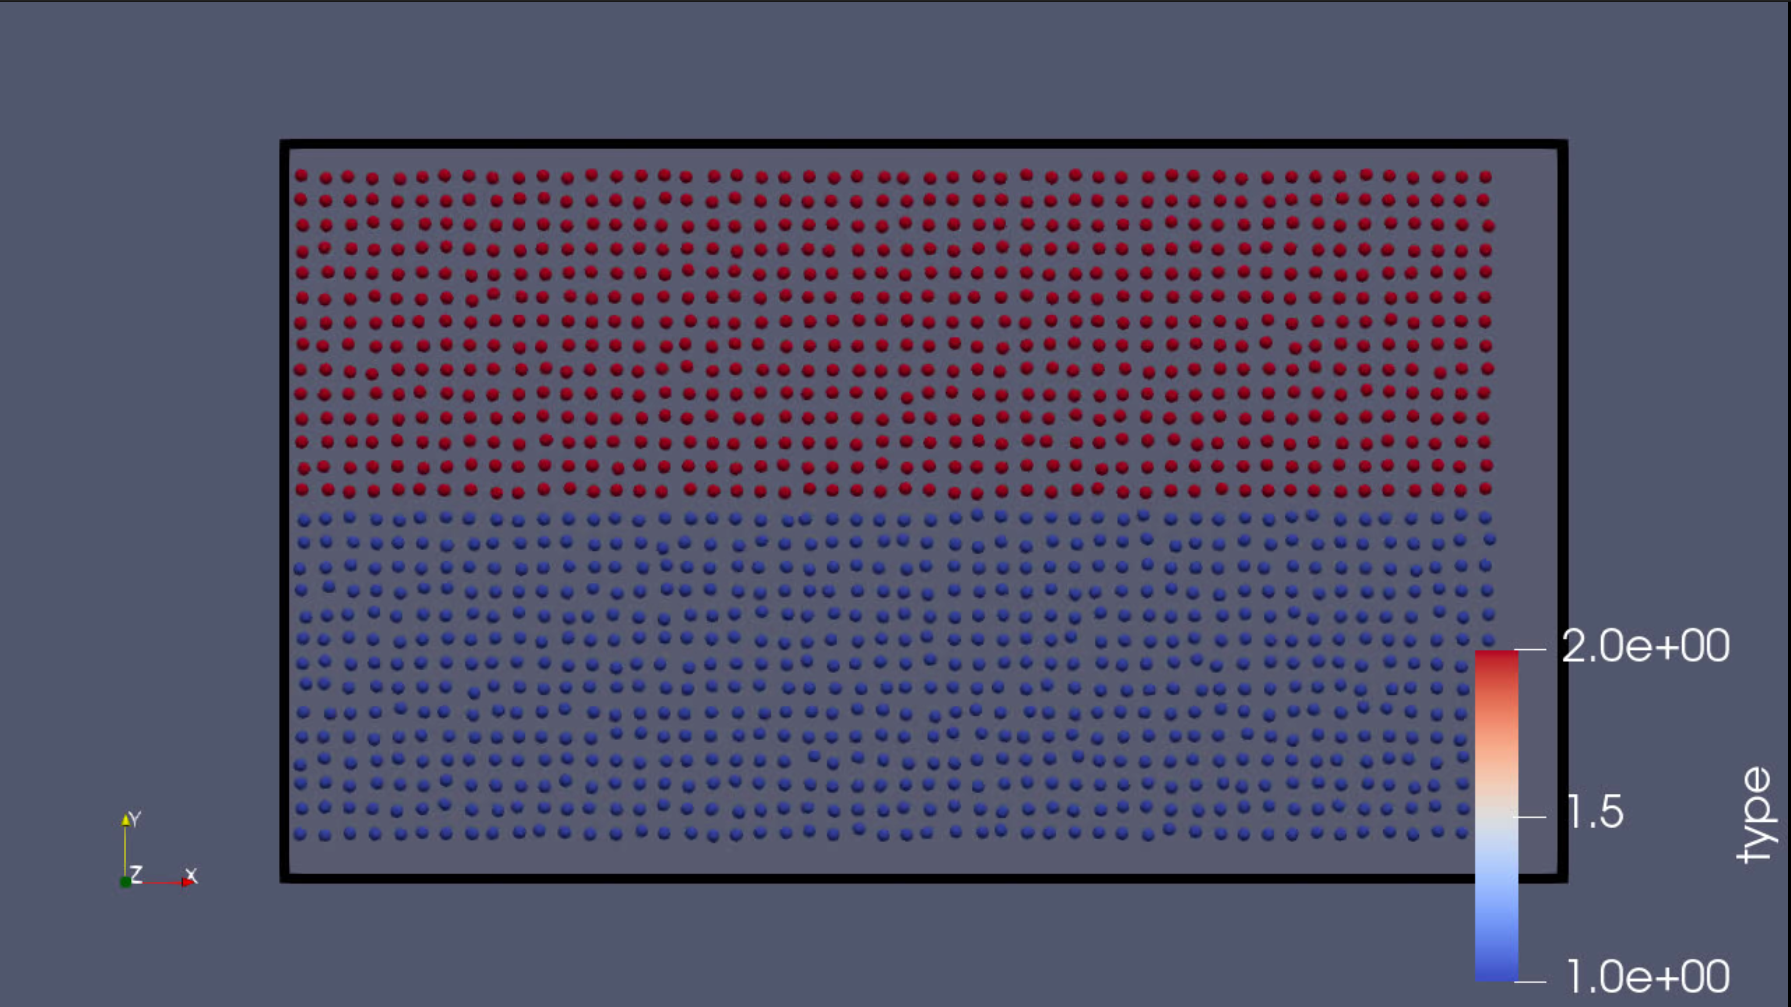
\includegraphics[width=0.7\textwidth]{small_rti.png}}{small_rti_broken.ogx}
		%\caption{caption}
	\end{figure} 
\end{frame}

\begin{frame}
	\frametitle{The problem}
	\large
	\begin{enumerate}
		\item Outer boxes may not have the expected sidelengths
		\item Interacting with neighbouring cells $\centernot \implies$ Catching everything in $r_{cutoff}$
	\end{enumerate}
	
			\begin{tikzpicture}[scale=1.3]
			%define constants
			\def\xLargeArrow{4.5}
			\def\yLargeArrow{1.5}
			\def\LargeArrowLength{2.5}
			\def\offSGrid{7.5}
			\def\arrowStart{0.6}
			\def\arrowEnd{1.9}
			
			\def\scale{1.4}
			
			%draw left grid
			\foreach \y in {0,...,2} {
				\filldraw [fill=green, draw=black] (0, \y) rectangle (0 + 1 ,\y + 1);
			}
			\foreach \x in {1,...,2}{
				\foreach \y in {0,...,2}{
					\draw [draw=black] (\x, \y) rectangle (\x +1 ,\y + 1);
				}
			}
			\foreach \y in {0,..., 2}{
				\draw [draw=black] (3, \y) rectangle (3 + 0.5,\y + 1);
			}
			
			\fill (0.2,1.4) circle[radius=2pt];
			\fill (2.8,1.4) circle[radius=2pt];
			
			%arrow in between
			\draw[->, line width = 1mm] (\xLargeArrow, \yLargeArrow) -- (\xLargeArrow + \LargeArrowLength, \yLargeArrow);
			
			
			%draw right grid with left row put to the right
			\foreach \y in {0,...,2} {
				\filldraw [fill=green, draw=black] (\offSGrid + 3 - 0.5, \y) rectangle (\offSGrid + 3 + 1 - 0.5,\y + 1);
			}
			\foreach \x in {0,...,1}{
				\foreach \y in {0,...,2}{
					\draw [draw=black] (\offSGrid + \x, \y) rectangle (\offSGrid + \x +1 ,\y + 1);
				}
			}
		
			\foreach \y in {0,..., 2}{
				\draw [draw=black] (\offSGrid + 2, \y) rectangle (\offSGrid + 2 + 0.5,\y + 1);
			}
			
			
			\fill (\offSGrid + 3 - 0.5 + 0.2,1.4) circle[radius=2pt];
			\fill (\offSGrid - 1 + 2.8,1.4) circle[radius=2pt];
			
			%arrows
			\draw[-triangle 60] (\offSGrid + 3.5 - 0.5, 1.5) -- (\offSGrid + 2.5 - 0.25, 1.5);
			\draw[-triangle 60] (\offSGrid + 3.5 - 0.5, 1.5) -- (\offSGrid + 2.5 - 0.25, 2.5);
			\draw[-triangle 60] (\offSGrid + 3.5 - 0.5, 1.5) -- (\offSGrid + 2.5 - 0.25, 0.5);
			
			
		\end{tikzpicture}
	
	$\implies$ Interact with one more "`Cellblock"' in that direction
\end{frame}

\begin{frame}
	\frametitle{Adding Periodic bounds}
	\large
	This slide should look very familiar to Assignment 3
		\begin{figure}
			\centering
			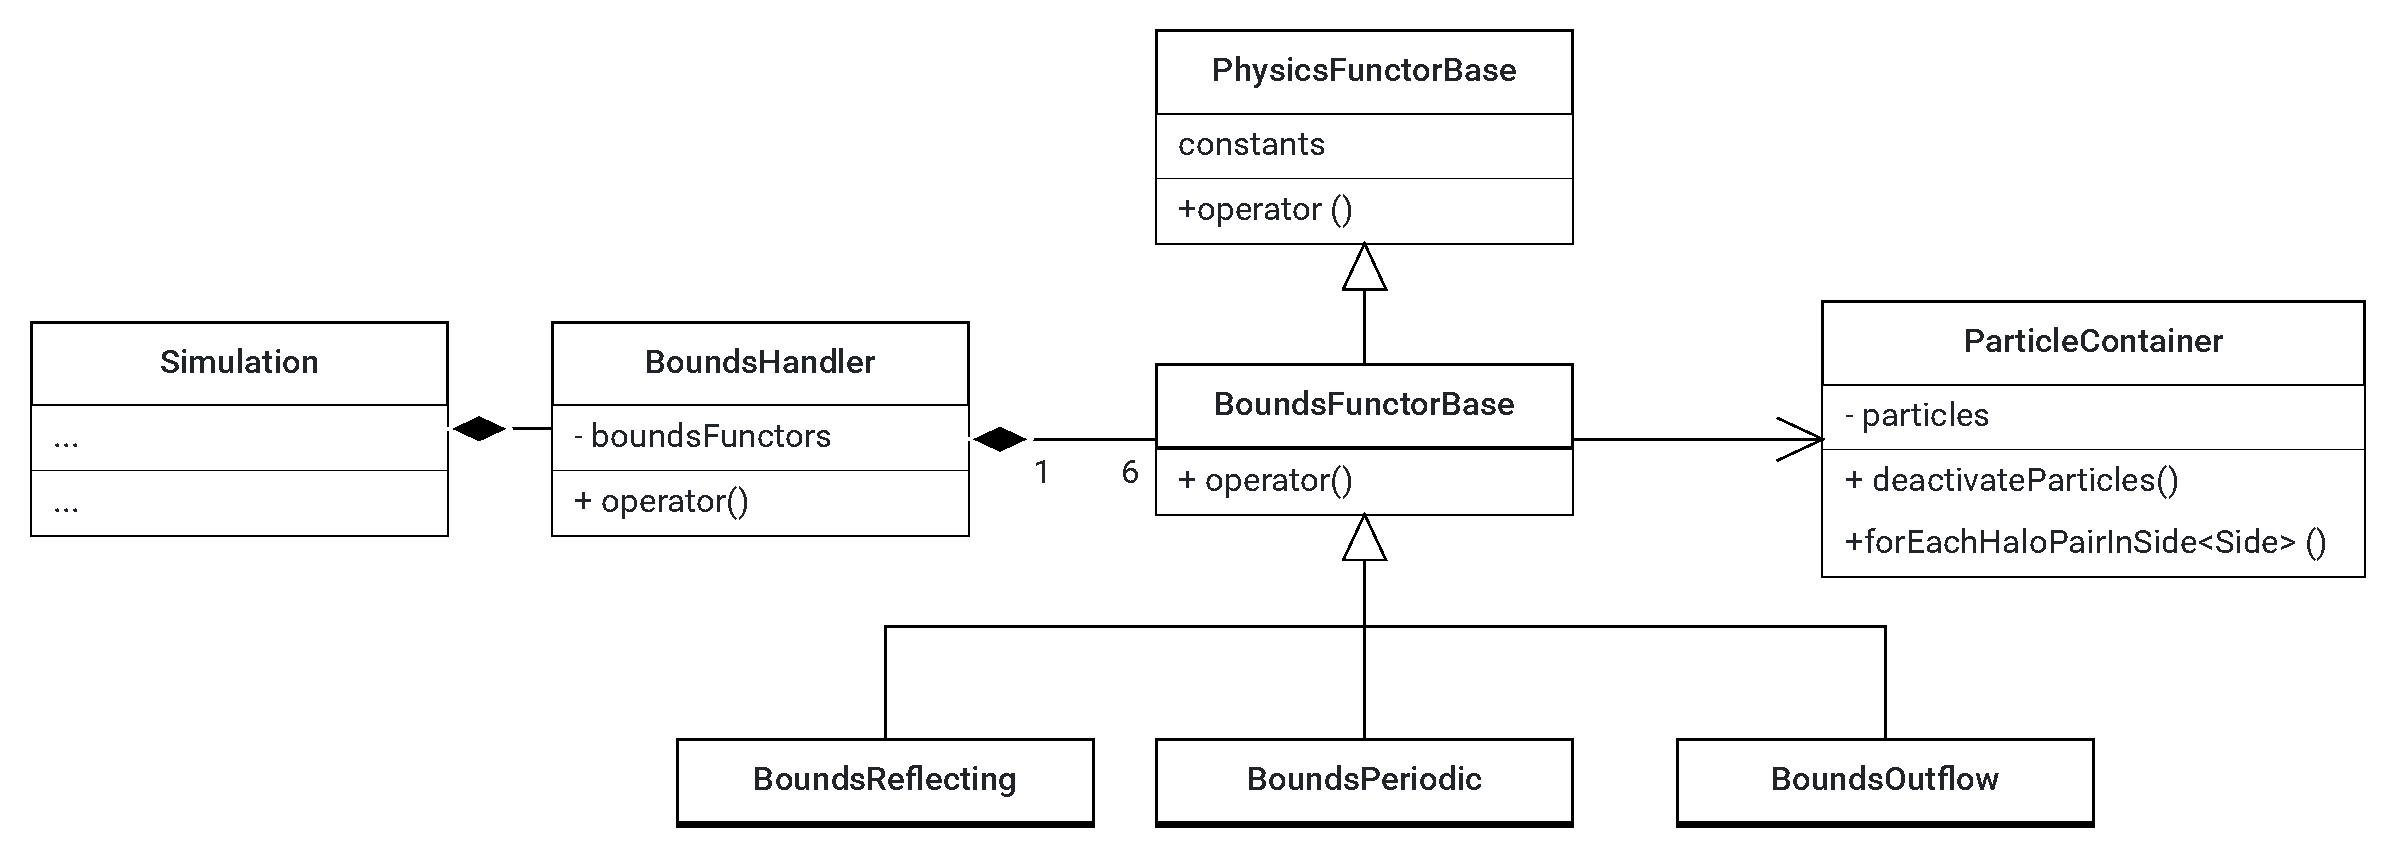
\includegraphics[width=0.95\linewidth]{BoundaryMolSim}
			\label{fig:boundarymolsim}
		\end{figure}
\end{frame}

\begin{frame}[fragile]
	\frametitle{Adding Gravitational Force}
	%\begin{columns}
	%	\begin{column}{0.5\textwidth}
			\begin{figure}
				\centering
				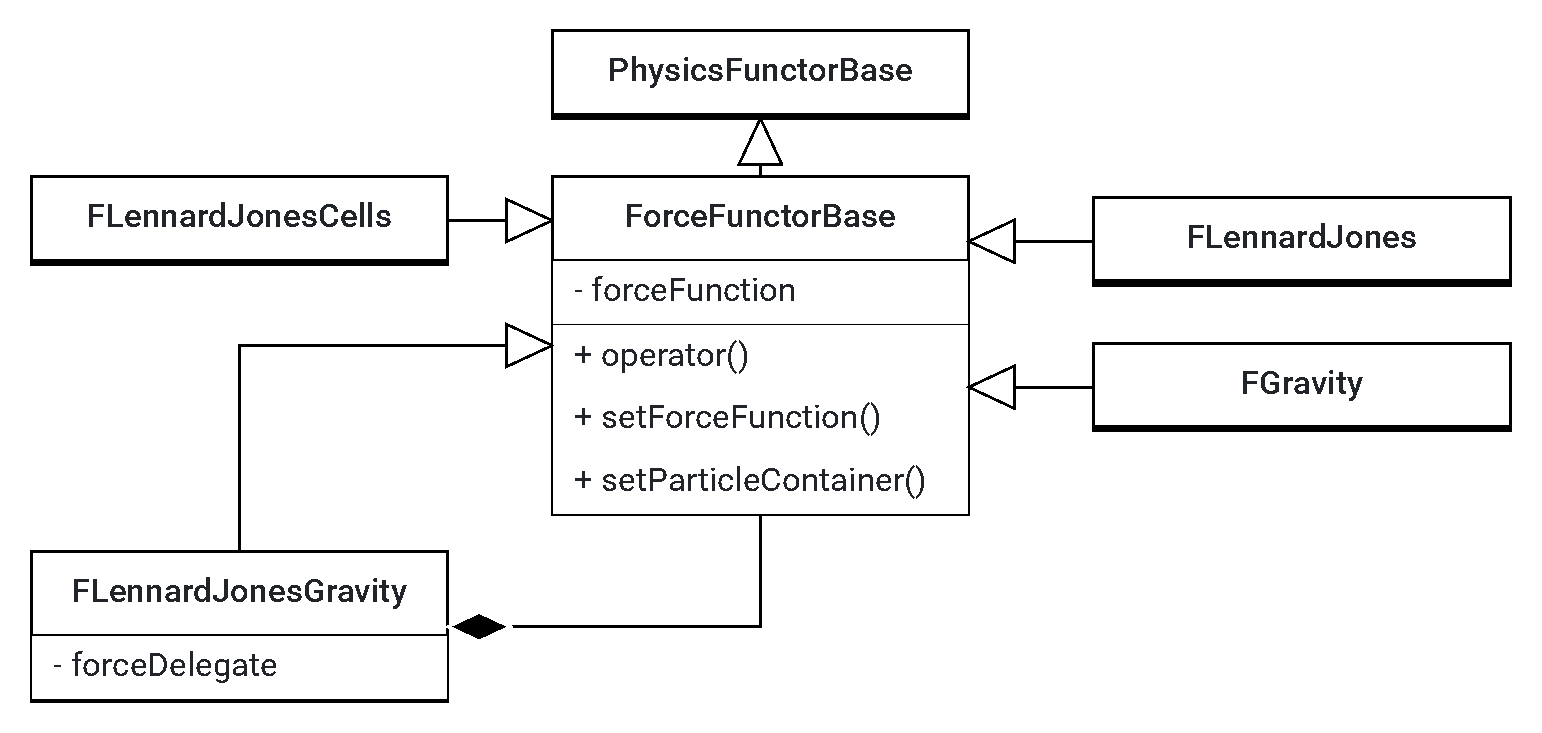
\includegraphics[width=0.6\linewidth]{FGravity_added}
				\label{fig:fgravityadded}
			\end{figure}
	%	\end{column}
	%\begin{column}{0.5\textwidth}
			
\begin{lstlisting}
		FLennardJonesGravity::operator()(){
			forceDelegate->operator()();
			particleContainer.forAllParticles([](auto& p){
			p.force[1] += p.m * gGrav;
			});	}
\end{lstlisting}

	%\end{column}
		
	%\end{columns}
	
\end{frame}

\begin{frame}[fragile]
	\frametitle{Optimizations 1}
	\large
As mentioned in Assignment 3 our ParticleContainer does not contain Particle-structs anymore.\\
Keeping the old interface lead to the following method:
\begin{lstlisting}
void ParticleContainer::forAllParticles(void(*function)(Particle &)) {
	for (unsigned long index: activeParticles) {
		Particle p;
		loadParticle(p, index);
		function(p);
		storeParticle(p, index);
	}
}
\end{lstlisting}

$\implies$ rewriting old code where this method got used was a major improvement

\end{frame}

\begin{frame}
	\frametitle{Optimizations 2}
	\large
	
	\begin{figure}
		\centering
		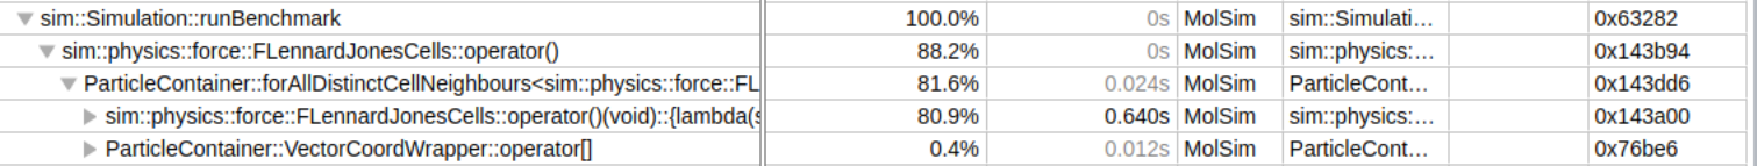
\includegraphics[width=1\linewidth]{profile_preoptimization_just_relevant_part}
		\label{fig:profilepreoptimizationjustrelevantpart}
	\end{figure}
	
	\begin{itemize}
		\item Force calculation takes a significant portion of CPU time
		\item Force between two particles in Force-Functors got represented as lambda expression
	\end{itemize}
	
	$\implies$ Represent force as static function instead
	
\end{frame}

\begin{frame}
	\frametitle{Small Rayleigh-Taylor instability}
	
	\begin{figure}[h!]
		\centering    
		\movie[label=show3,width=0.70\textwidth,poster
		,autostart,showcontrols,loop] 
		{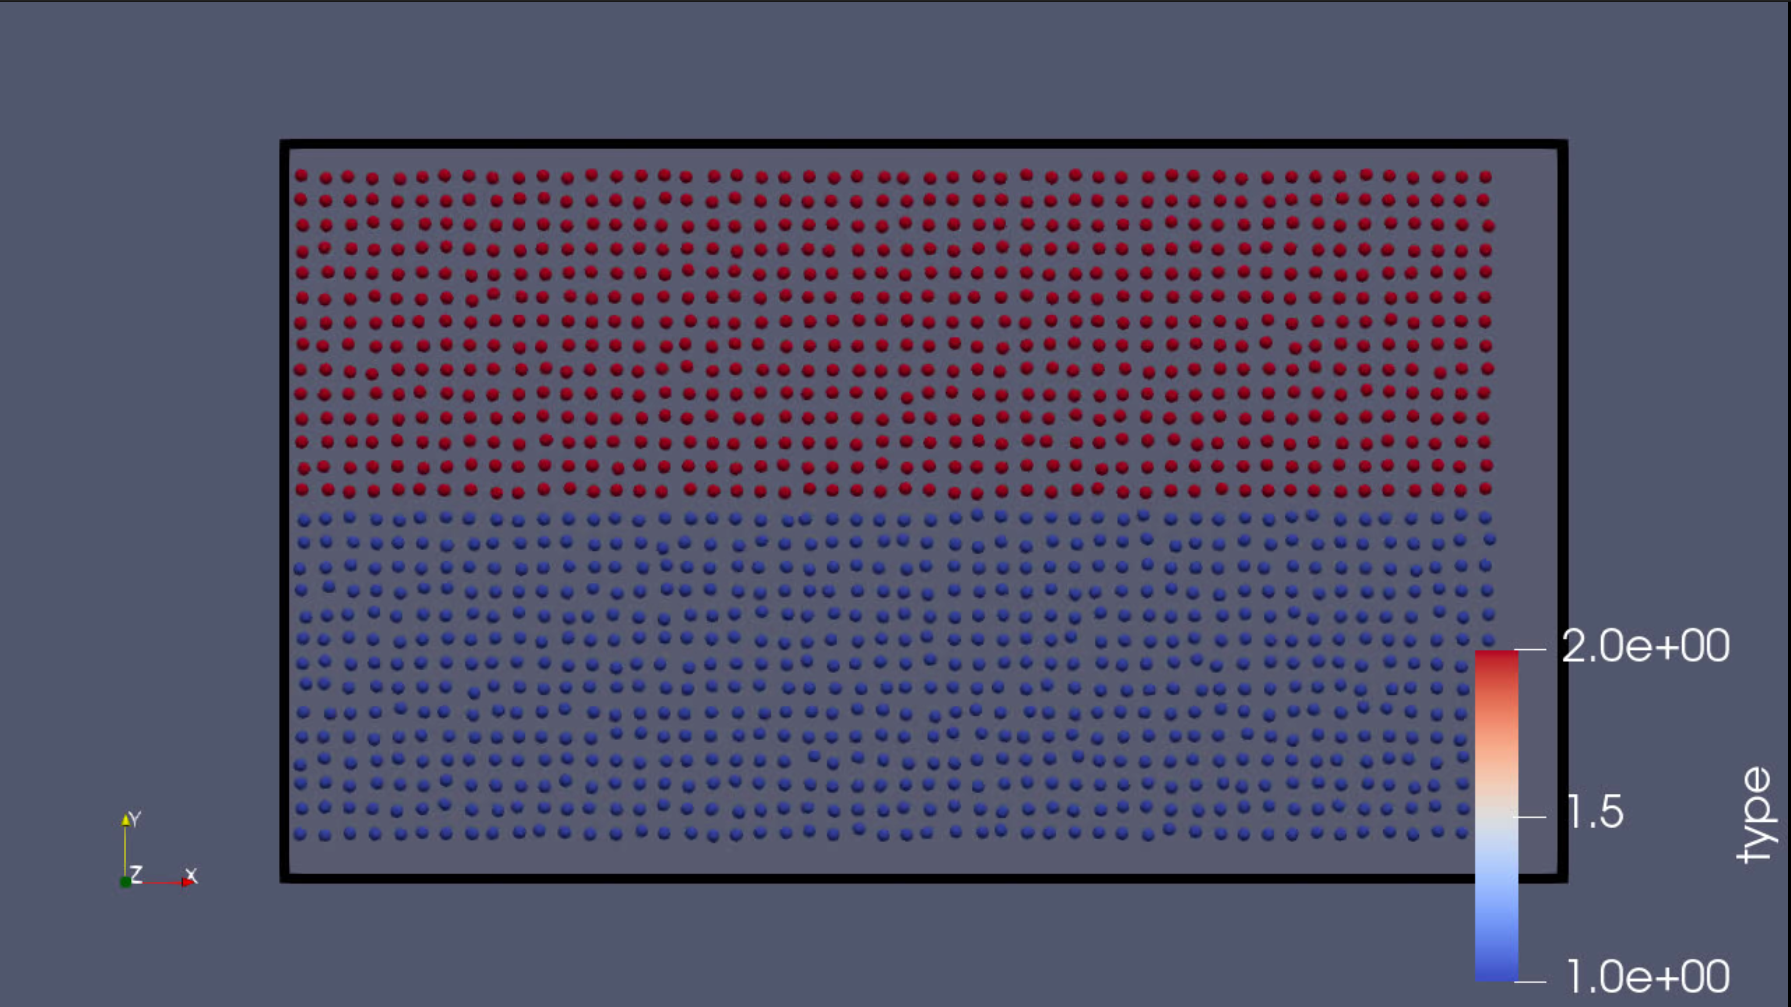
\includegraphics[width=0.70\textwidth]{small_rti.png}}{small_rti.mp4}
		%\caption{caption}
	\end{figure} 
	
\end{frame}

\begin{frame}
	\frametitle{Rayleigh-Taylor instability}
	\begin{figure}[h!]
		\centering    
		\movie[label=show3,width=0.75\textwidth,poster
		,autostart,showcontrols,loop] 
		{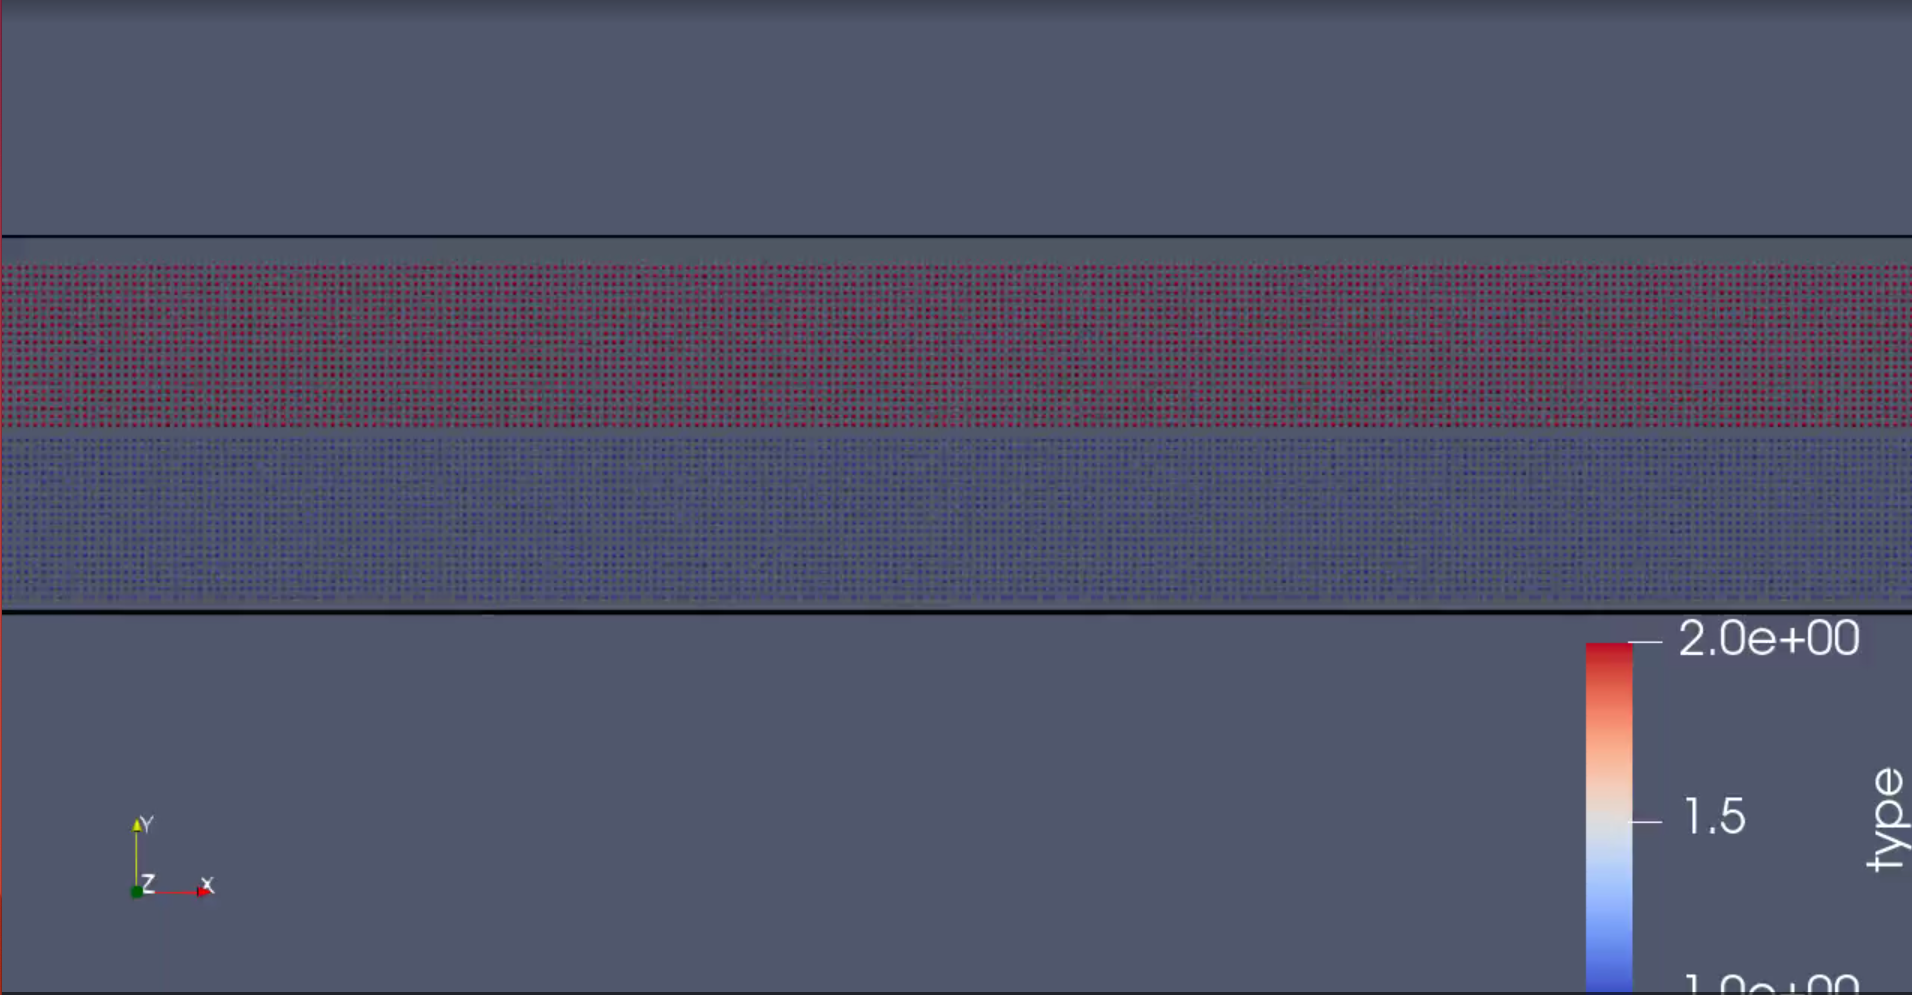
\includegraphics[width=0.75\textwidth]{large_rti.png}}{large_rti.mp4}
		%\caption{caption}
	\end{figure} 
\end{frame}

\begin{frame}
	\frametitle{Falling drop}
	\begin{figure}[h!]
		\centering    
		\movie[label=show3,width=0.70\textwidth,poster
		,autostart,showcontrols,loop] 
		{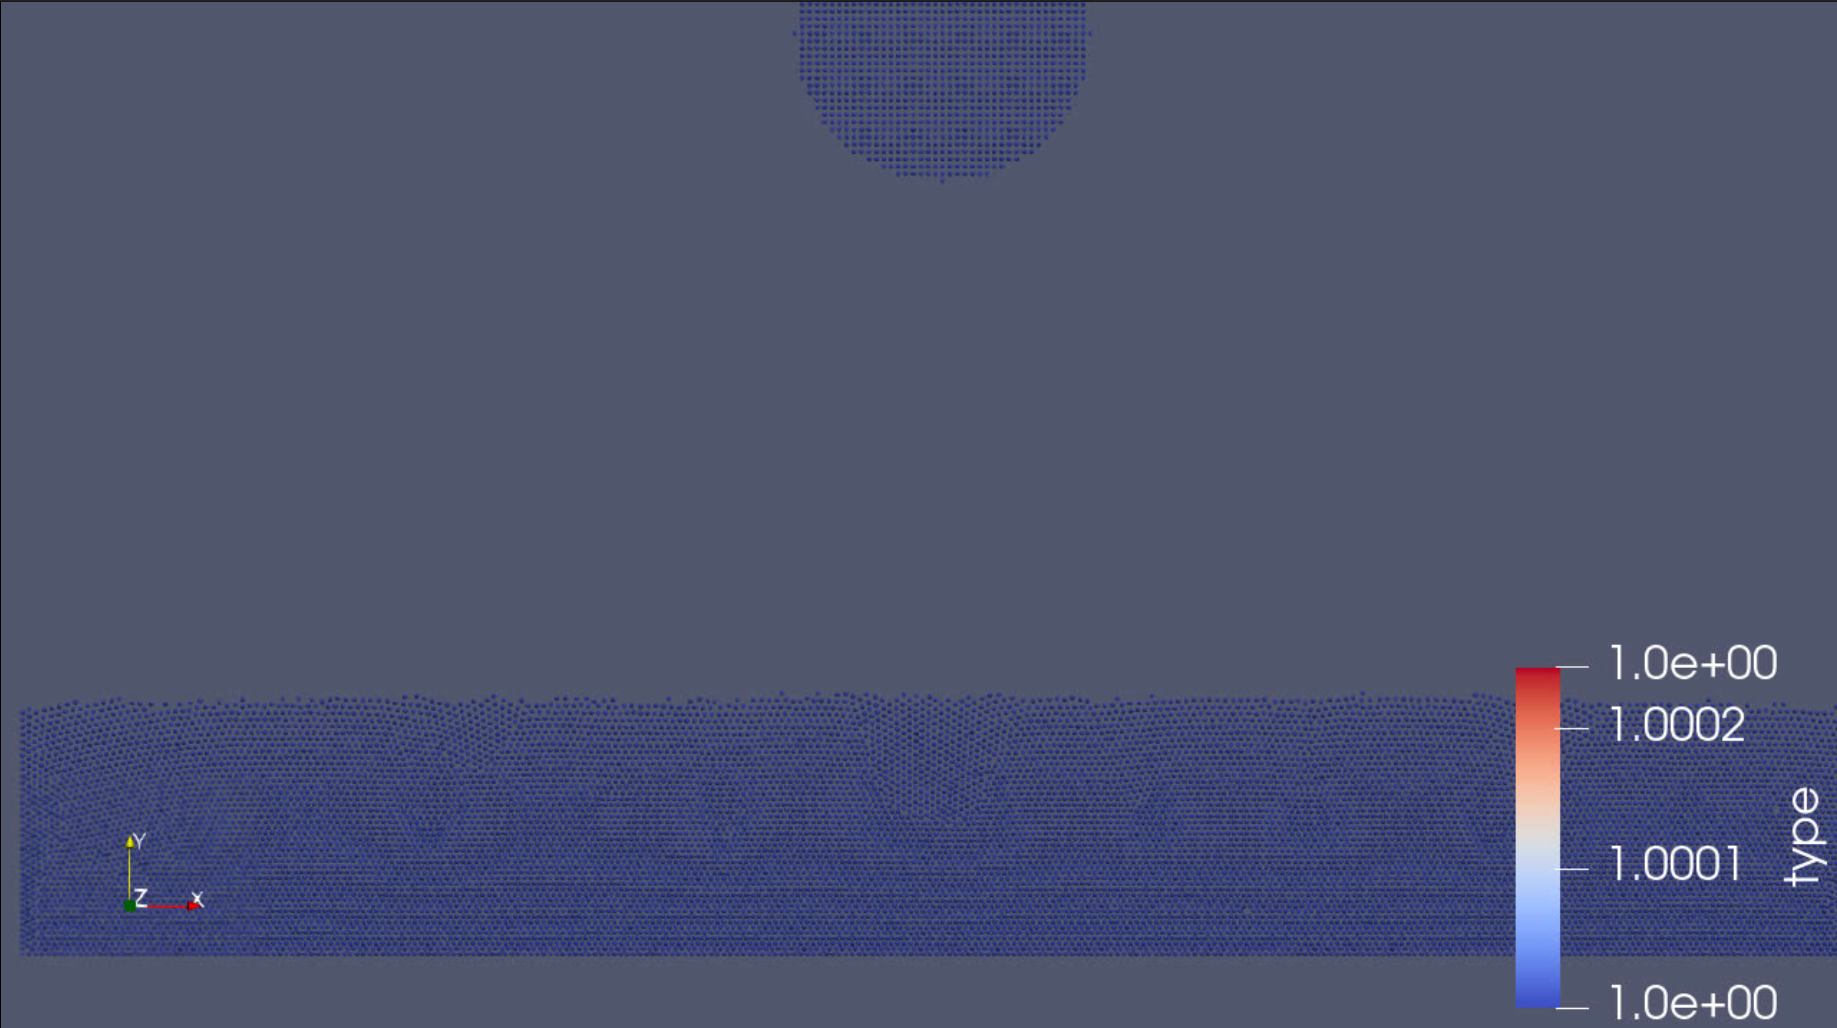
\includegraphics[width=0.70\textwidth]{falling_drop.png}}{falling_drop_out.mp4}
		%\caption{caption}
	\end{figure} 
\end{frame}

\begin{frame}
	\frametitle{Serial Benchmarks}
	\large
	\begin{itemize}
		\item As already mentioned building with the Intel compiled didn't work even with major time investments
		\item The option "`-slow"' lets the code run in the pre-optimized state
	\end{itemize}
	
	\Large
	\centering
	\begin{tabular}{lll}
		Options   & MMU/s Cluster & MMU/s Local\\
		-slow -O2 & $0.0087$ & $\geq 1/6 \cdot 0.036\  \land \leq 1/2 \cdot 0.036$ \\
		-O2 	  & $0.0087$ & $0.036$\\
		-O0 	  & $0.0087$ & $0.036$\\	
	\end{tabular}

	\large
	Since these measurements are so close together and significantly smaller than our local measurements, we assume that something went wrong on the cluster.

\end{frame}

\begin{frame}
	\frametitle{Roadblocks}
	\large
	\begin{itemize}
		\item Compiling and running jobs on the cluster turned out to be a nightmare
		\item Intel compiler broke us trying to unbreak him
		\item Searching for bugs that may or may not be there (bouncy particles in Rayleigh-Taylor)
		\item Searching for bugs that definitely are there (see Boundary conditions)
		\item Large time investments in order to get tools to run
	\end{itemize}
\end{frame}

\begin{frame}
	\PraesentationBildUhrenturm
	%\PraesentationStartseiteFlaggen
\end{frame}

\begin{frame}
	\frametitle{Recreating Profiling}
	\large
	\begin{enumerate}
		\item \texttt{mkdir build}
		\item \texttt{cmake ..}
		\item \texttt{make ProfileMolSim} or \texttt{make CXX\_FLAGS+="-Dslow -std=c++20" ProfileMolSim}
		\item  \texttt{./ProfileMolSim ../input/[file\_you\_want\_to\_profile]}
		\item  \texttt{gprof ProfileMolSim gmon.out > profile-data.txt}
	\end{enumerate}
\end{frame}


%\frame[label=blah]{
%	\begin{center}%
%		\href{run:/usr/local/bin/mplayer -fs standard-benchmark.mp4}{
%		\includegraphics[scale=0.25]
%		{Assignment2_Presentation.pdf}}

%		\includemovie{.85\textheight}{.85\textheight}{standard-benchmark.mp4}%
%	\end{center}%
%	\note{%
%		\begin{itemize}
%			\item blah
%			\item blah
%		\end{itemize}
%	}%
%}


%%%%%%%%%%%%%%%%%%%%%%%%%%%%%%%%%%%%%%%%%%%%%%%%%%%%%
%% Folie: Gültigkeit der Masterfolien              %%
%%%%%%%%%%%%%%%%%%%%%%%%%%%%%%%%%%%%%%%%%%%%%%%%%%%%%
